\documentclass[a4paper,12pt]{article}
\usepackage{graphicx}
\usepackage{verbatim}
\usepackage{amsmath}
\usepackage{listings}
\usepackage{xcolor}
\begin{document}
	\title{\textbf{Homework2 Rostagno File2}}
	\author{295706}
	\date{\today}
	\maketitle
	
	\centering \textbf{Esercizio 1}\\
	\begin{itemize}
		\item \textbf{Punto 1:}
		Come prima cosa genero tramite runif() le due cordinate per ogni punto $\textbf{s}$ e le salvo in una matrice.\\
		Mostro tramite plot grafico i 100 punti ottenuti
		\begin{figure}[h] % L'ambiente figure permette di gestire il posizionamento
			\centering % Centra l'immagine
			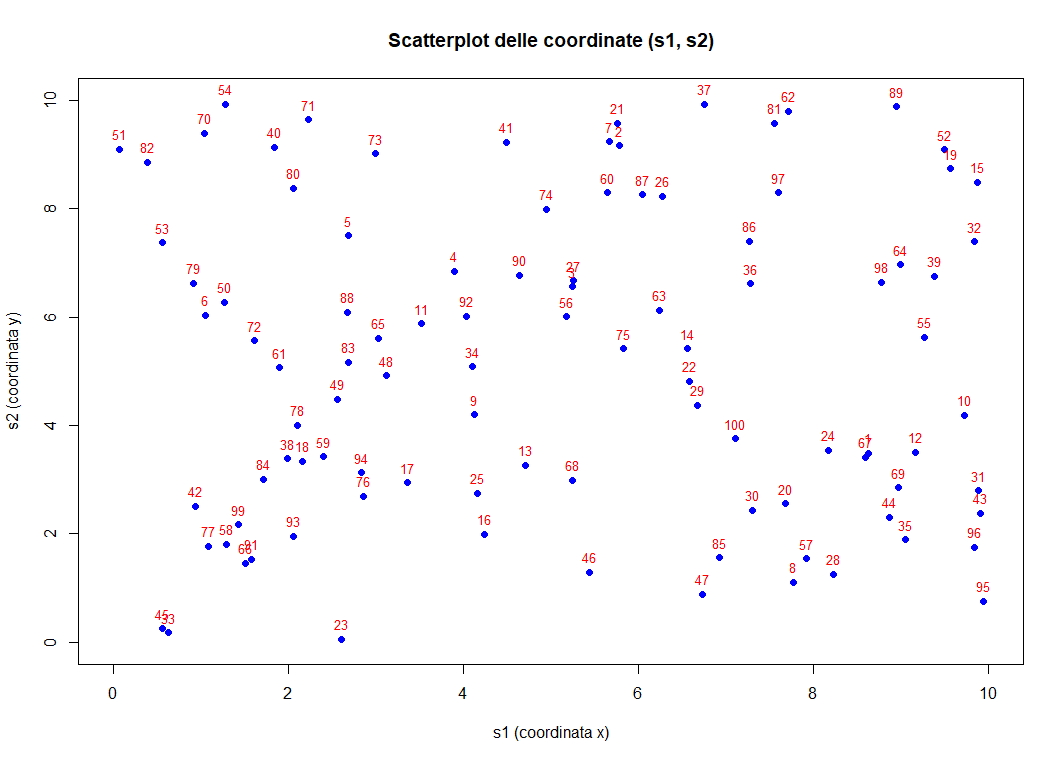
\includegraphics[width=0.8\textwidth]{punti.png} % Inserisce l'immagine con larghezza metà pagina
			\caption{Osservazioni effettuate } % Aggiunge una didascalia all'immagine
			\label{fig:immagine} % Aggiunge un'etichetta per riferimenti interni
		\end{figure}
		\newline
		Successivamente calcolo la matrice di covarianza applicando la formula data nel modello e calcolando le distanza come una matrice dove in ogni posizione é indicata la distanza tra il punto $s_i$ e il punto $s_j$.\\
		Ora posso campionare W come campione di una normale multi variata tramite il comando mvrnorm().\\
		Infine trattandosi di un processo gaussiano possiamo scrivere Y come:
		\[
		Y(s)=W(s)+\epsilon_i 
		\]
		Dove $\epsilon \sim \mathcal{N}(0, \tau^2)$ e quindi campionarlo.
		\item \textbf{Punto 2:}
		Calcolo i quartili e li salvo in un vettore tramite il comando quantile().\\
		Successivamente creo un vettore "colore" inizializzato con il rosso per ogni osservazione y. Ora verifico ogni osservazione a quale quartile appartiene e ne modifico il colore nel vettore "colore". \\
		Infine eseguo uno scatterplot delle osservazioni e imposto la voce colore con il set creato precedentemente ottenendo dunque
		\begin{figure}[h] % L'ambiente figure permette di gestire il posizionamento
			\centering % Centra l'immagine
			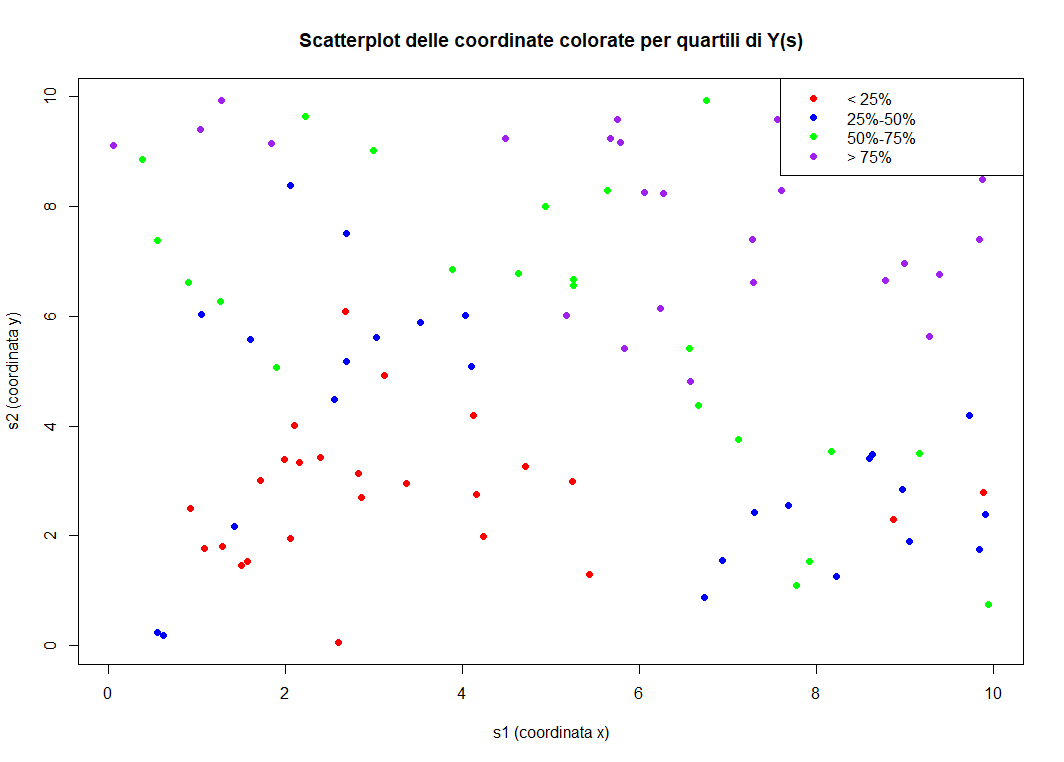
\includegraphics[width=0.8\textwidth]{colore.png} % Inserisce l'immagine con larghezza metà pagina
			\caption{Quartili delle osservazioni } % Aggiunge una didascalia all'immagine
			\label{fig:immagine} % Aggiunge un'etichetta per riferimenti interni
		\end{figure}
		\item \textbf{Punto 3:}
		Come numero casuale ho ottenuto il 66, successivamente ho generato un indice casuale per decidere quali osservazioni ($Y_o$), quali coordinate($D_o$) e quali valori ($W_o$) mantenere per utilizzarli nel campionamento delle full-conditional.\\
		Devo svolgere un algoritmo MCMC per ottenere campioni da
		\[
		f(\beta_0,\beta_1,\tau^2,\sigma^2,\phi | y_0,w_0)
		\]
		Ho iniziato impostando 5000 iterate per l'algoritmo di Gibbs e inizializzando i vari parametri secondo le indicazioni fornite nell'homework.\\
		Come prior dei vari parametri ho utilizzato:
		\begin{itemize}
			\item $\beta_0 \sim \text{N}(0, 1000)$: in modo da non essere esplicativa
			\item $\beta_1 \sim \text{N}(0, 1000)$: in modo da non essere esplicativa
			\item $\tau^2 \sim \text{IG}(1, 1)$: inverted gamma
			\item $\sigma^2 \sim \text{IG}(1, 1)$: inverted gamma
			\item $\phi \sim \text{U}(\frac{3}{\text{max dist}}, \frac{3}{\text{min dist}})$: uniforme
		\end{itemize}
		Dove max dist e min dist sono i valori di distanza minima e massima tra le coordinate di $D_o$.\\
		Successivamente ho creato dei vettori $samples \_ nome$ per memorizzare i valori che verranno assunti dai parametri durante l'algoritmo.\\
		Durante ogni iterata ho cosí deciso di campionare i vari parametri:
		\begin{itemize}
			\item \textbf{Campionamento di $\beta_0$}\\
			Per trovare la full conditional di \( \beta_0 \), ho considerato solo i termini di \( f(\beta_0,\beta_1,\tau^2,\sigma^2,\phi , y_0,w_0) \) che dipendono da \( \beta_0 \). Gli altri termini possono essere ignorati, poiché non influenzano il campionamento. Ottengo:
			\[
			f(\beta_0|\beta_1,\tau^2,\sigma^2,\phi , y_0,w_0) \sim f(\omega_o | \beta_0,\beta_1,\sigma^2,\phi)*f(\beta_0)
			\]
			Dove la verosomiglianza é
			\[
			f(w_0 \mid \beta_0, \beta_1, \phi) \propto |C|^{-\frac{1}{2}} \exp \left( -\frac{1}{2} (w_0 - m )^T C^{-1} (w_0 - m) \right),
			\]
			Con $m=\beta_0 1 + \beta_1 s_1$.\\
			Mentre $\beta_0 \sim N(\mu_{\beta_0},\tau_{\beta_0})$ in generale vale:
			\[
			f(\beta_0) \propto \exp \left( -\frac{1}{2\tau_{\beta_0}^2} (\beta_0 - \mu_{\beta_0})^2 \right).
			\]
			Combiniamole assieme eliminando i termini che non hanno dipendenza e otteniamo
			\[
			f(\beta_0 \mid \dots) \propto \exp \left( 
			-\frac{1}{2} \left[
			\beta_0^2 \left( \mathbf{1}^T C^{-1} \mathbf{1} + \frac{1}{\tau_{\beta_0}^2} \right) \right. \right.
			\]
			\[
			\left. \left. 
			- 2\beta_0 \left( \mathbf{1}^T C^{-1} (\mathbf{w}_o - \beta_1 \mathbf{s}_1) 
			+ \frac{\mu_{\beta_0}}{\tau_{\beta_0}^2} \right)
			\right]
			\right).
			\]
			
			
			Confrontiamo con la forma generale di una normale:
			\[
		    \quad 
			\exp \left( -\frac{1}{2} a \beta_0^2 + b \beta_0 \right) \sim \mathcal{N} \left( -\frac{b}{a}, \frac{1}{a} \right).
			\]
			
			\begin{enumerate}
				\item \textbf{Varianza della posteriori:}
				\[
				\sigma_{\beta_0}^2 = \left( \mathbf{1}^T C^{-1} \mathbf{1} + \frac{1}{\tau_{\beta_0}^2} \right)^{-1}.
				\]
				
				\item \textbf{Media della posteriori:}
				\[
				\mu_{\beta_0} = -\sigma_{\beta_0}^2 \left( \mathbf{1}^T C^{-1} (\mathbf{w}_o - \beta_1 \mathbf{s}_1) + \frac{\mu_{\beta_0}}{\tau_{\beta_0}^2} \right).
				\]
			\end{enumerate}
			\item \textbf{Campionamento di $\beta_1$}\\
			Per trovare la full conditional di \( \beta_1 \), ho considerato solo i termini di \( f(\beta_0,\beta_1,\tau^2,\sigma^2,\phi , y_0,w_0) \) che dipendono da \( \beta_1 \). Gli altri termini possono essere ignorati, poiché non influenzano il campionamento. Ottengo:
			\[
			f(\beta_1|\beta_0,\tau^2,\sigma^2,\phi , y_0,w_0) \sim f(\omega_o | \beta_0,\beta_1,\sigma^2,\phi)*f(\beta_1)
			\]
			Dove la verosomiglianza é
			\[
			f(w_0 \mid \beta_0, \beta_1, \phi) \propto |C|^{-\frac{1}{2}} \exp \left( -\frac{1}{2} (w_0 - m )^T C^{-1} (w_0 - m) \right),
			\]
			Con $m=\beta_0 1 + \beta_1 s_1$.\\
			Mentre $\beta_1 \sim N(\mu_{\beta_1},\tau_{\beta_1})$ in generale vale:
			\[
			f(\beta_0) \propto \exp \left( -\frac{1}{2\tau_{\beta_1}^2} (\beta_1 - \mu_{\beta_1})^2 \right).
			\]
			Combiniamole assieme eliminando i termini che non hanno dipendenza e otteniamo
			\[
			f(\beta_1 \mid \beta_0, \mathbf{w}_o, \phi) \propto \exp \left( 
			-\frac{1}{2} \left[ 
			\beta_1^2 \mathbf{s}_1^T C^{-1} \mathbf{s}_1 
			- 2\beta_1 \left( \mathbf{s}_1^T C^{-1} \mathbf{w}_o - \beta_0 \mathbf{1}^T C^{-1} \mathbf{s}_1 \right)
			\right] \right)
			\]
			\[
			\cdot \exp \left( 
			-\frac{1}{2\tau_{\beta_1}^2} \left[ 
			\beta_1^2 - 2\mu_{\beta_1} \beta_1
			\right] \right).
			\]
			Confrontiamo con la forma generale di una normale:
			\[
			\exp \left( -\frac{1}{2} a \beta_1^2 + b \beta_1 \right) \sim \mathcal{N} \left( -\frac{b}{a}, \frac{1}{a} \right).
			\]
			
			
			1. Varianza della posteriori:
			\[
			\sigma_{\beta_1}^2 = \left( \mathbf{s}_1^T C^{-1} \mathbf{s}_1 + \frac{1}{\tau_{\beta_1}^2} \right)^{-1}.
			\]
			
			2. Media della posteriori:
			\[
			\mu_{\beta_1} = -\sigma_{\beta_1}^2 \cdot \left( 
			\mathbf{s}_1^T C^{-1} \mathbf{w}_o - \beta_0 \mathbf{1}^T C^{-1} \mathbf{s}_1 + \frac{\mu_{\beta_1}}{\tau_{\beta_1}^2} 
			\right).
			\]
			
			\item \textbf{Campionamento di $\tau^2$}\\
			Per trovare la full conditional di \( \tau^2 \), ho considerato solo i termini di \( f(\beta_0,\beta_1,\tau^2,\sigma^2,\phi , y_0,w_0) \) che dipendono da \( \tau^2 \). Gli altri termini possono essere ignorati, poiché non influenzano il campionamento. Ottengo:
			\[
			f(\tau^2|\beta_0,\beta_1,\sigma^2,\phi , y_0,w_0) \sim f(y_0 | w_0,\tau^2)*f(\tau^2)
			\]
			Dove la verosomiglianza é
			\[
			f(\mathbf{y}_o \mid \mathbf{w}_o, \tau^2) \propto (\tau^2)^{-\frac{n}{2}} 
			\exp \left( -\frac{1}{2 \tau^2} (\mathbf{y}_o - \mathbf{w}_o)^T (\mathbf{y}_o - \mathbf{w}_o) \right).
			\]
			Mentre $\tau^2 \sim IG(a_{\tau},b_{\tau})$
			\[
			f(\tau^2) \propto (\tau^2)^{-(a_{\tau}+1)} exp(-\frac{b_{\tau}}{\tau^2})
			\]
			Combiniamole assieme eliminando i termini che non hanno dipendenza e otteniamo
			\[
			f(\tau^2 \mid \mathbf{w}_o, \mathbf{y}_o) \propto (\tau^2)^{-\frac{n}{2}} 
			\exp \left( -\frac{1}{2 \tau^2} (\mathbf{y}_o - \mathbf{w}_o)^T (\mathbf{y}_o - \mathbf{w}_o) \right)
			\]
			\[
			\cdot (\tau^2)^{-(a_\tau + 1)} \exp \left( -\frac{b_\tau}{\tau^2} \right).
			\]
			
			Quindi come posteriori avremo
			\[
			\tau^2 \mid \dots \sim IG \left( a_\tau + \frac{n}{2}, \, b_\tau + \frac{1}{2} (\mathbf{y}_o - \mathbf{w}_o)^T (\mathbf{y}_o - \mathbf{w}_o) \right).
			\]
			\item \textbf{Campionamento di $\sigma^2$}\\
			Per trovare la full conditional di \( \sigma^2 \), ho considerato solo i termini di \( f(\beta_0,\beta_1,\tau^2,\sigma^2,\phi , y_0,w_0) \) che dipendono da \( \sigma^2 \). Gli altri termini possono essere ignorati, poiché non influenzano il campionamento. Ottengo:
			\[
			f(\sigma^2|\beta_0,\tau^2,\beta_1,\phi , y_0,w_0) \sim f(\omega_o | \beta_0,\beta_1,\sigma^2,\phi)*f(\sigma^2)
			\]
			Dove la verosomiglianza é
			\[
			f(w_0 \mid \beta_0, \beta_1, \phi, \sigma^2) \propto |C|^{-\frac{1}{2}} \exp \left( -\frac{1}{2} (w_0 - m )^T C^{-1} (w_0 - m) \right),
			\]
			Con $m=\beta_0 1 + \beta_1 s_1$.\\
			Mentre $\sigma^2 \sim IG(a_{\sigma},b_{\sigma})$
			\[
			f(\sigma^2) \propto (\sigma^2)^{-(a_{\sigma}+1)} exp(-\frac{b_{\sigma}}{\sigma^2})
			\]
			Combiniamole assieme eliminando i termini che non hanno dipendenza e otteniamo
			\[
			f(\sigma^2 \mid \dots) \propto (\sigma^2)^{-\frac{n}{2}} 
			\exp \left( -\frac{1}{2 \sigma^2} (\mathbf{w}_o - m)^T R^{-1} (\mathbf{w}_o - m) \right)
			\]
			\[
			\cdot (\sigma^2)^{-(a_\sigma + 1)} \exp \left( -\frac{b_\sigma}{\sigma^2} \right).
			\]
			Con $m=\beta_0 1 + \beta_1 s_1$\\
			e $R=exp(-\phi*distances)$.\\
			Quindi come posteriori avremo
			\[
			\sigma^2 \mid \dots \sim IG \left( 
			a_\sigma + \frac{n}{2}, \, 
			b_\sigma + \frac{1}{2} (\mathbf{w}_o - m)^T R^{-1} (\mathbf{w}_o - m)
			\right).
			\]
			\item \textbf{Campionamento di $\phi$}\\
			Per trovare la full conditional di \( \phi \), ho considerato solo i termini di \( f(\beta_0,\beta_1,\tau^2,\sigma^2,\phi , y_0,w_0) \) che dipendono da \( \phi \). Gli altri termini possono essere ignorati, poiché non influenzano il campionamento. Ottengo:
			\[
			f(\beta_1|\beta_0,\tau^2,\sigma^2,\phi , y_0,w_0) \sim f(\omega_o | \beta_0,\beta_1,\sigma^2,\phi)*f(\phi)
			\]
			Dove la verosomiglianza é
			\[
			f(w_0 \mid \beta_0, \beta_1, \phi) \propto |C|^{-\frac{1}{2}} \exp \left( -\frac{1}{2} (w_0 - m )^T C^{-1} (w_0 - m) \right)
			\]
			Con $m=\beta_0 1 + \beta_1 s_1$.\\
			Mentre $\phi \sim U(a_{\phi},b_{\phi})$
			\[
			f(\phi) \propto \frac{1}{b_{\phi}-a_{\phi}}
			\]
			Combiniamole assieme eliminando i termini che non hanno dipendenza e otteniamo
			\[
			f(\phi \mid \dots) \propto |C|^{-\frac{1}{2}} \exp \left( -\frac{1}{2} (w_0 - m )^T C^{-1} (w_0 - m) \right) \cdot \frac{1}{b_{\phi}-a_{\phi}}
			\]
			Ma purtroppo non riusciamo a dedurre nessuna forma chiusa, quindi per campionare $\phi$ utilizzeremo Metropolis-Hasting.\\
			Come distribuzione proposal per il parametro $\phi^*$ proposto utilizzo
			\[
			\phi^* \sim N(\phi,\eta)
			\]
			Quindi centrata nel valore corrente di $\phi$ e come varianza inizializzata a 1.\\
			Successivamente la varianza verrá modificata ogni 50 iterazioni secondo la formula
			\[
			\eta_{new}=exp(log(\eta) + \frac{100}{200+t}*(mean \_ alpha - 0.25))
			\] 
			Dove mean$\_$alpha é la media dei 50 coefficenti alpha di accettazione.\\
			Ora proponiamo un nuovo valore $\phi^*$ il quale deve appartenere al dominio $\phi \in [\frac{3}{\text{max dist}}, \frac{3}{\text{min dist}}]$ mostrato precedentemente e calcoliamo il rapporto di accettazione $\alpha$ come:
			\[
			\alpha = \min \left( 1, \,
			\frac{f(\phi^* \mid \dots) \, q(\phi \mid \phi^*)}
			{f(\phi \mid \dots) \, q(\phi^* \mid \phi)} \right),
			\]
			\[
			\text{dove:}
			\]
			\begin{itemize}
				\item $f(\phi^* \mid \dots)$: La full conditional di $\phi^*$,
				\item $f(\phi \mid \dots)$: La full conditional di $\phi$,
				\item $q(\phi^* \mid \phi)$: La distribuzione di proposta.
			\end{itemize}
			
			Siccome la proposta $q(\phi^* \mid \phi)$ è simmetrica (ad esempio, una normale centrata su $\phi$), il rapporto di proposta si cancella:
			
			\[
			\frac{q(\phi \mid \phi^*)}{q(\phi^* \mid \phi)} = 1.
			\]
			
			Abbiamo che:
			\[
			f(\phi^* \mid \dots) \propto |C(\phi^*)|^{-\frac{1}{2}}
			\exp \left( 
			-\frac{1}{2} (W - \mu)^T C(\phi^*)^{-1} (W - \mu)
			\right),
			\]
			
			\[
			f(\phi \mid \dots) \propto |C(\phi)|^{-\frac{1}{2}}
			\exp \left( 
			-\frac{1}{2} (W - \mu)^T C(\phi)^{-1} (W - \mu)
			\right).
			\]
			
			Come da suggerimento calcoleremo questo valore come $exp^{log(\alpha)}$ quindi otteniamo che
			\begin{align*}
				\log(\alpha) = 
				& -\frac{1}{2} \left[ \log(|C(\phi^*)|) + (W - \mu)^T C(\phi^*)^{-1} (W - \mu) \right] \\
				& + \frac{1}{2} \left[ \log(|C(\phi)|) + (W - \mu)^T C(\phi)^{-1} (W - \mu) \right].
			\end{align*}
			Quindi possiamo proseguire in questa maniera per calcolare $\alpha$ cercando di evitare la cancellazione numerica
			\begin{enumerate}
				\item \textbf{Log-determinante}: Calcoliamo $\log(|C(\phi^*)|)$ e $\log(|C(\phi)|)$ usando la funzione determinante:
				\[
				\text{log-det-term} = \frac{1}{2} \left[ \log(|C(\phi)|) - \log(|C(\phi^*)|) \right].
				\]
				
				\item \textbf{Termine quadratico}: Calcoliamo la differenza nei termini quadratici:
				\[
				\text{quad-term} = \frac{1}{2} \left[ (W - \mu)^T C(\phi^*)^{-1} (W - \mu) - (W - \mu)^T C(\phi)^{-1} (W - \mu) \right].
				\]
				
				\item \textbf{Logaritmo di $\alpha$}: Combiniamo i due termini:
				\[
				\log(\alpha) = \text{log-det-term} + \text{quad-term}.
				\]
				
				\item \textbf{Calcolo di $\alpha$}: Passiamo dalla scala logaritmica a quella esponenziale:
				\[
				\alpha = \min(1, \exp(\log(\alpha))).
				\]
			\end{enumerate}
		\end{itemize}
			Una volta ottenuto il valore $\alpha$ non ci resta che simulare $u \sim U(0,1)$ e accettare $\alpha$ se $u\leq\alpha$ oppure in caso negativo mantenere lo stesso valore di $\phi$.\\
			Ora effettuo il burn-in di 1000 simulazioni per stabilizzare la convergenza.\\
			Infine osservo tramite plot grafico l'evolversi dei parametri.
			\begin{figure}[h] % L'ambiente figure permette di gestire il posizionamento
				\centering % Centra l'immagine
				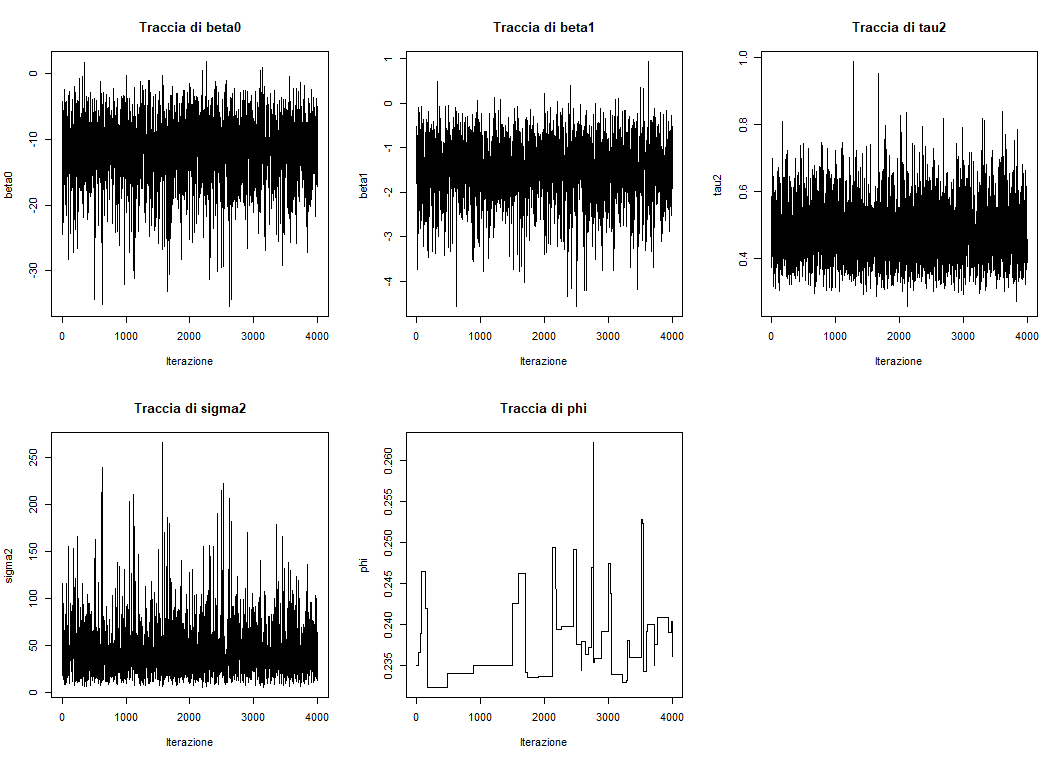
\includegraphics[width=0.8\textwidth]{mcmc1.png} % Inserisce l'immagine con larghezza metà pagina
				\caption{Evolversi del campionamento dei vari parametri} % Aggiunge una didascalia all'immagine
				\label{fig:immagine} % Aggiunge un'etichetta per riferimenti interni
			\end{figure}
		
	\end{itemize}
	\centering \textbf{Esercizio 2}\\
	\begin{itemize}
		\item \textbf{Punto 1:}
		Come primo passo ho simulato il campione $\textbf{z}$ generando un vettore di lunghezza $n$ dove in ogni sua posizione puó contenere i valori $1,2,3$ con probabilità $\pi$ (ho utilizzato il comando sample()). \\
		Successivamente ho campionato le osservazioni $y$ come campione di una Poisson di parametro $\lambda_1,\lambda_2 \text{o}\lambda_3$ in base al valore corrispettivo di $z_i$ (comando rpois()).\\
		Successivamente ho rappresentato tramite grafico le varie osservazioni ottenute divise per colore in base al parametro $\lambda$ con cui sono state osservate. Sull'asse x  sono presenti gli indici delle osservazioni (1:n) mentre sull'asse delle y sono presenti i valori assunti da ogni osservazione.\\
		\begin{figure}[h] % L'ambiente figure permette di gestire il posizionamento
			\centering % Centra l'immagine
			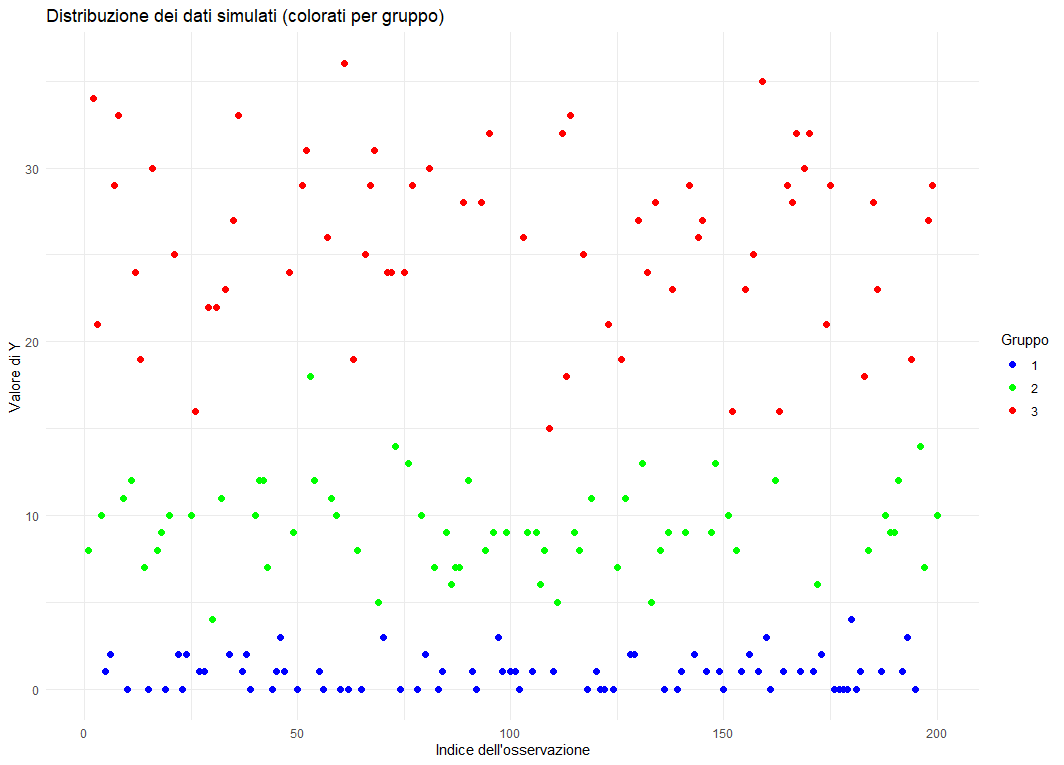
\includegraphics[width=0.7\textwidth]{scatter_oss_pois.png} % Inserisce l'immagine con larghezza metà pagina
			\caption{Osservazioni effettuate divise per gruppo} % Aggiunge una didascalia all'immagine
			\label{fig:immagine} % Aggiunge un'etichetta per riferimenti interni
		\end{figure}
		\newpage
		Successivamente ho rappresentato tramite istogramma il numero di osservazioni di ogni gruppo per osservare se il campionamento di $\textbf{z}$ ha rispettato le varie probabilità (ovviamente la somma delle tre colonne é n).
		\begin{figure}[h] % L'ambiente figure permette di gestire il posizionamento
			\centering % Centra l'immagine
			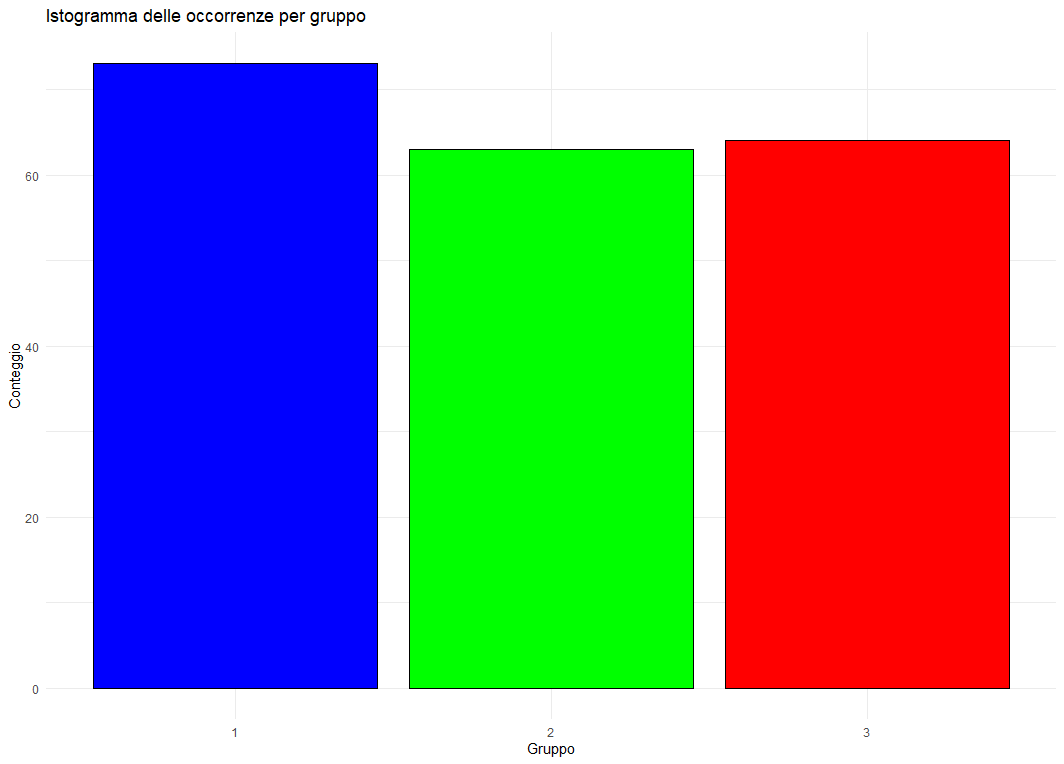
\includegraphics[width=0.6\textwidth]{isto.png} % Inserisce l'immagine con larghezza metà pagina
			\caption{Numero di osservazioni di ogni gruppo} % Aggiunge una didascalia all'immagine
			\label{fig:immagine} % Aggiunge un'etichetta per riferimenti interni
		\end{figure}
		\newpage
		\item \textbf{Punto 2:}
		Inizialmente ho assunto delle prior per i vari parametri in modo che fossero abbastanza neutrali (non devono dare troppa informazione a priori ai parametri):\\
		\begin{itemize}
			\item $\lambda_k \sim \text{Gamma}(1, 1)$: Parametro inizialmente non informativo.
			\item $\pi \sim \text{Dirichlet}(1, 1, 1)$: Distribuzione uniforme sui tre gruppi.
		\end{itemize}
		Successivamente ho creato delle matrici chiamate $samples \_ nome$ per contenere i valori dei vari parametri durante le varie iterazioni dell'algoritmo MCMC.\\
		Come algoritmo ho utilizzato il solito Gibbs sampler:\\
		\begin{itemize}
			\item Come prima cosa ho inizializzato i vari parametri tramite le prior sopra definite, mentre per $z$ ho generato un vettore con sample() senza definire delle probabilità.
			\item Successivamente ho impostato un ciclo di 1000 iterate dove ad ogni iterata campionavo i parametri z,lambda e pi e salvavo i risultati nelle matrici.
			\item \textbf{Campionamento di z}\\
			Per trovare la full conditional di \( z_i \), ho considerato solo i termini di \( f(y, z, \lambda, \pi) \) che dipendono da \( z_i \). Gli altri termini possono essere ignorati, poiché non influenzano il campionamento. Ottengo:
			\[
			f(z_i = k \mid y, \lambda, \pi) \propto f(z_i = k) \cdot P(y_i \mid \lambda_k)= \pi_k \cdot P(y_i \mid \lambda_k)
			\]
			Espandendo i termini:
			\[
			f(z_i = k \mid y, \lambda, \pi) \propto \pi_k \cdot \frac{\lambda_k^{y_i} e^{-\lambda_k}}{y_i!}
			\]
			Dove:
			\begin{itemize}
				\item \( \pi_k \) è la proporzione del gruppo \( k \).
				\item \( P(y_i \mid \lambda_k) = \frac{\lambda_k^{y_i} e^{-\lambda_k}}{y_i!} \) è la probabilità di osservare \( y_i \) dato il parametro del gruppo \( k \).
			\end{itemize}
			Poiché il termine \( \frac{1}{y_i!} \) è costante rispetto a \( z_i \), possiamo ignorarlo per il campionamento:
			\[
			f(z_i = k \mid y, \lambda, \pi) \propto \pi_k \cdot \lambda_k^{y_i} e^{-\lambda_k}
			\]
			Siccome il vettore $\pi$ deve avere che la somma delle sue componenti sia uguale a 1, dobbiamo normalizzare il risultato in questo modo:\\
			\[
			P(z_i = k \mid y, \lambda, \pi) = \frac{\pi_k \cdot \lambda_k^{y_i} e^{-\lambda_k}}{\sum_{j=1}^{K} \pi_j \cdot \lambda_j^{y_i} e^{-\lambda_j}}
			\]
			Ora non mi resta che creare un ciclo for che per ogni osservazione $y_i$ calcola questo vettore di probabilità (lunghezza 3 in questo caso, una per ogni $\lambda$) e genera sempre tramite sample() il valore $z_i$ corrispondente.\\
			Al termine del ciclo for avró il mio campione di $\textbf{z}$.
			\item \textbf{Campionamento di lambda}\\
			Per trovare la full conditional di $\lambda_k$, considero solo i termini di $f(y, z, \lambda, \pi)$ che dipendono da $\lambda_k$:
			\[
			f(\lambda_k \mid y, z, \pi) \propto f(\lambda_k) \cdot \prod_{i:z_i=k} P(y_i \mid \lambda_k).
			\]
			La prior di $\lambda_k$ è una distribuzione Gamma:
			\[
			f(\lambda_k) \propto \lambda_k^{\alpha_k - 1} e^{-\beta_k \lambda_k}.
			\]
			La verosomiglianza per $y_i$ nel gruppo $k$ è Poisson:
			\[
			P(y_i \mid \lambda_k) = \frac{\lambda_k^{y_i} e^{-\lambda_k}}{y_i!}.
			\]
			Unendo prior e verosomiglianza:
			\[
			f(\lambda_k \mid y, z, \pi) \propto \lambda_k^{\alpha_k - 1} e^{-\beta_k \lambda_k} \cdot \prod_{i:z_i=k} \lambda_k^{y_i} e^{-\lambda_k}.
			\]
			Espandendo i termini:
			\[
			f(\lambda_k \mid y, z, \pi) \propto \lambda_k^{\alpha_k - 1 + \sum_{i:z_i=k} y_i} e^{-(\beta_k + n_k) \lambda_k}.
			\]
			Dove:
			\[
			n_k = \sum_{i:z_i=k} 1 \quad \text{: numero di osservazioni nel gruppo } k,
			\]
			\[
			\sum_{i:z_i=k} y_i \quad \text{: somma delle osservazioni assegnate al gruppo } k.
			\]
			La full conditional di $\lambda_k$ è una distribuzione Gamma:
			\[
			f(\lambda_k \mid y, z, \pi) \sim \text{Gamma}\left(\alpha_k + \sum_{i:z_i=k} y_i, \, \beta_k + n_k\right).
			\]
			Ora non mi resta che impostare un ciclo for di lunghezza 3 e calcolare un campione con il comando rgamma() per ogni $\lambda$ e salavrli tutti e 3 nella mia matrice.
			\item \textbf{Campionamento di pi}\\
			Per trovare la full conditional di $\pi$, considero solo i termini che dipendono da $\pi$:
			\[
			f(\pi \mid y, z, \lambda) \propto f(\pi) \cdot \prod_{i=1}^n \prod_{k=1}^K \pi_k^{1_{z_i=k}}.
			\]
			
			Espandendo:
			\begin{itemize}
				\item La prior di $\pi$ è una Dirichlet:
				\[
				f(\pi) \propto \prod_{k=1}^K \pi_k^{\alpha_k - 1}.
				\]
				
				\item Il termine legato a $z$ è:
				\[
				\prod_{i=1}^n \prod_{k=1}^K \pi_k^{1_{z_i=k}} = \prod_{k=1}^K \pi_k^{n_k},
				\]
				dove $n_k = \sum_{i=1}^n 1_{z_i=k}$ è il numero di osservazioni assegnate al gruppo $k$.
			\end{itemize}
			
			Combinando prior e verosomiglianza:
			\[
			f(\pi \mid y, z, \lambda) \propto \prod_{k=1}^K \pi_k^{\alpha_k - 1 + n_k}.
			\]
			
			La full conditional di $\pi$ è una distribuzione Dirichlet:
			\[
			f(\pi \mid y, z, \lambda) \sim \text{Dirichlet}(\alpha_1 + n_1, \alpha_2 + n_2, \dots, \alpha_K + n_K).
			\]
			Adesso semplicemente campione un vettore di probabilità con il comando rdichlet() .\\
			Ovviamente come campione di z utilizzo l'ultimo campione appreso e non quello iniziale(come viene indicato dall'algoritmo di Gibbs).
		\end{itemize}
		Una volta terminato l'algoritmo effettuo il burn-in dei primi 200 elementi poiché rovinano la convergenza.\\
		Eseguo alcuni plot grafici ed osservo l'evolversi dei parametri $\lambda$ e $\pi$
		\begin{figure}[h] % L'ambiente figure permette di gestire il posizionamento
			\centering % Centra l'immagine
			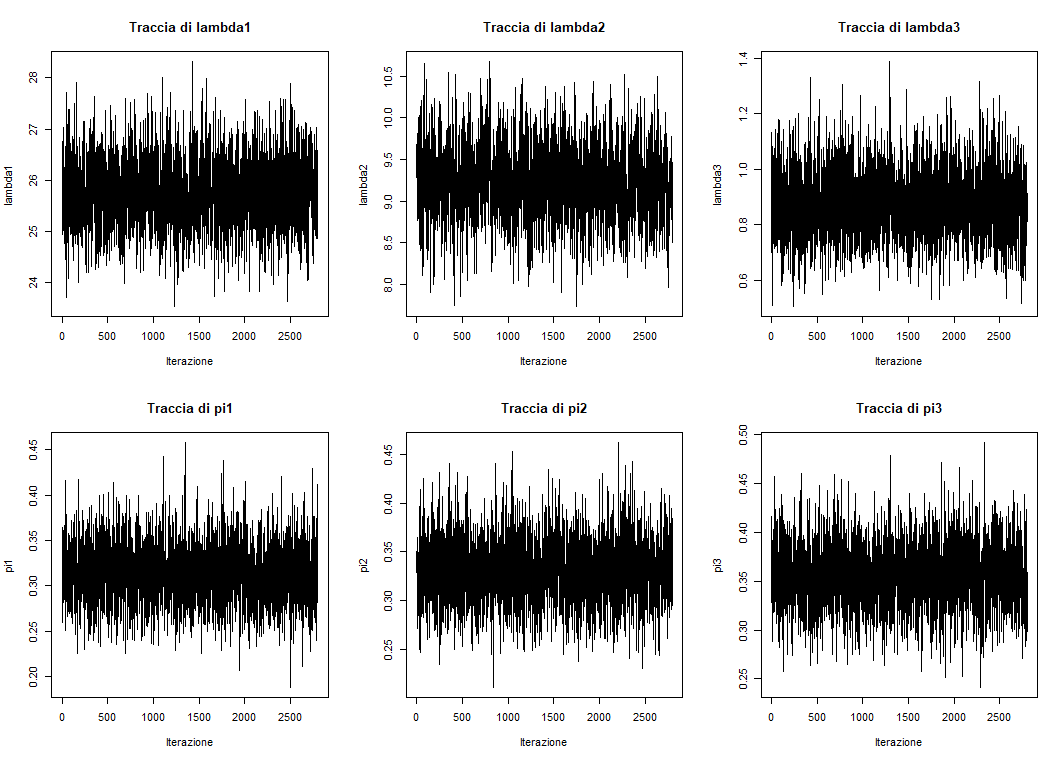
\includegraphics[width=1.1\textwidth]{plotfinali2.png} % Inserisce l'immagine con larghezza metà pagina
			\caption{Osservazioni di ogni parametro} % Aggiunge una didascalia all'immagine
			\label{fig:immagine} % Aggiunge un'etichetta per riferimenti interni
		\end{figure}
	\end{itemize}
	
\end{document}